\clearpage
\title{Implementing \& Plotting Taylor Series for Sine in MATLAB}
\author{}
\date{}
\maketitle

\section*{Introduction}
\subsection*{Taylor Series}
The Taylor series is a way to represent a function as an infinite sum of terms calculated from the values of the function's derivatives at a specific point.\\\\
For a function \(f(x)\) that is infinitely differentiable at a point \(a\), the Taylor series expansion around \(a\) is given by:
\[f(x) = f(a) + f'(a)(x-a) + \frac{f''(a)}{2!}(x-a)^2 + \frac{f'''(a)}{3!}(x-a)^3 + \ldots
\]
For sine function, the taylor series is expanded as:
\[\sin(x) = x - \frac{x^3}{3!} + \frac{x^5}{5!} - \frac{x^7}{7!} + \ldots\]

\section*{Tools Used}
\begin{itemize}
    \item MATLAB R2021a - for writing and running code.
    \item MacTeX -\LaTeX  compiler.
    \item VS Code with \LaTeX workshop extension as a text editor.
\end{itemize}

\section*{Process}
\subsection*{Code for Taylor sine series:}
\begin{minted}[breaklines, linenos]{matlab}
    close all;
    clear all;
    clc;
    syms x;
    f =input('Enter the function : ');

    theta = -pi:pi/20:pi;

    g = f;

    %hold on;
    y = input('Enter the value for approximation: ');
    a = input('Enter the starting point: ');

    n = input('Enter the number of order: ');

    taylor = eval(subs(f,x,a));

    for i = 1:n
        f = diff(f,x);
        taylor = taylor + ( eval(subs(f,x,a)) * power((x-a),i) / factorial(i) );
        disp(taylor);
        plot(theta,subs(taylor,x,theta));
        hold on;
        if i == n
        plot(theta,subs(g,x,theta));
        end
    end

    disp(eval(subs(taylor,x,y)));
\end{minted}
\subsection*{Output}
\begin{center}
    \centering
    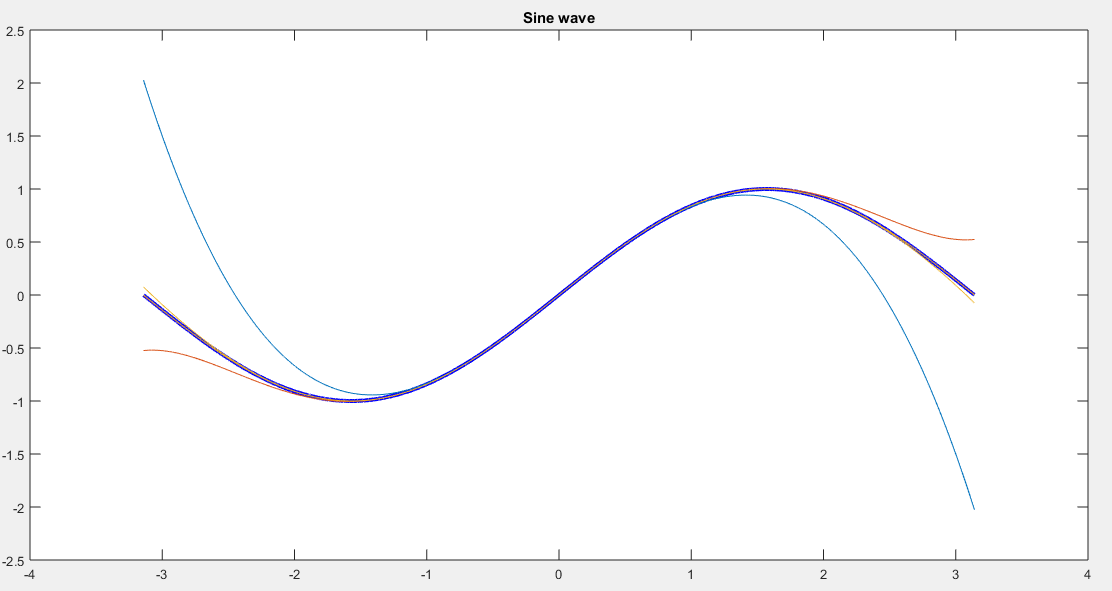
\includegraphics[width = .9\textwidth]{tay.png}
    \captionof{figure}{Taylor Sine Series ($-\pi \leq \:\: $x$ \:\: \leq \pi$)}
\end{center}



